\SourceLeaf{267}%
\Needspace{13\baselineskip}
8. Durch Verbindung von 3) und 4) ergibt sich die Relation:
\[
\tag*{III.} \sin B \,.\, da - \cos B\, g(a) \,.\, db - f(c) \,.\, dA = 0,
\]
aus der durch gleichzeitige Vertauschung von $a$ mit $b$ und $A$ mit $B$:
\[
\tag*{IV.} \cos A \,.\, db - \cos A\, g(b) \,.\, da - f(c) \,.\, dB = 0
\]
hervorgeht.

9. Aus I. und III. erhält man durch Elimination von $dA$ die Gleichung:
\[
\cos B \,.\, da + g(a) \sin B \,.\, db - dc = 0.
\]
Ebenso ist auch
\[
\cos A \,.\, db + g(b) \sin A \,.\, da - dc = 0,
\]
folglich muss
\[
(\cos B - g(b) \sin A)\, da + (\cos A - g(a) \sin B)\, db = 0
\]
sein. Da aber $da$ und $db$ von einander unabhängig sind, so ist das nur möglich,
wenn gleichzeitig
\[
\tag*{V. 1)} \cos A = g(a) \sin B,
\]
\[
\tag*{V. 2)} \cos B = g(b) \sin A
\]
wird. Aus diesen Gleichungen folgt die Relation:
\[
\tag*{V.} \cos B \,.\, da + \cos A \,.\, db - dc = 0.
\]

10. Verfährt man wie in No. 3, so ist in dem unendlich kleinen Dreieck $BB'D$
(Fig. 4):
\[
\tag*{5)} da = \cos B \,.\, dc,
\]
während $dA = 0$ wird. Verfährt man aber wie in No. 4, so ist in dem unendlich
kleinen Dreieck $BB'D$ (Fig. 5):
\[
\tag*{6)} da = \sin B\, f(c) \,.\, dA,
\]
während $dc = 0$ wird. Mithin ergibt die Verbindung von 5) und 6) die allgemein
gültige Formel:
\[
\tag*{VI.} da - \cos B \,.\, dc - \sin B\, f(c) \,.\, dA = 0,
\]
und entsprechend ist:
\[
\tag*{VII.} db - \cos A \,.\, dc - \sin A\, f(c) \,.\, dB = 0.
\]

\Needspace{37\baselineskip}
11. Man verlängere $CA$ um $AA' = db$ und trage in $A'$ an $CA'$ den Winkel $A$
an, dessen anderer Schenkel die Verlängerung der Kathete $CB$ in $B'$ schneide,
sodass $BB' = da$ wird. Von $A$ fälle man auf $A'B'$ das Lot $AD$ 
und trage auf $A'B'$ nach $B'$ hin $DE = c$ ab. Dann wird $A'D = \cos A \,.\, db$,
und da nach Fig. 8 und Gleichung V.:
\[
\begin{aligned}dc &= A'D + EB'\\ &= \cos B \,.\, da + \cos A \,.\, db\end{aligned}
\]
ist, $EB' = \cos B \,.\, da$, folglich $BE = \sin B \,.\, da$. Das Viereck $ADEB$
hat aber in $A$ und $D$ rechte Winkel, während $AB = DE = c$ ist, mithin ist nach
(A):
\[
BE = g(c) \,.\, AD
\]
oder
\[
\sin B \,.\, da = g(c) \sin A \,.\, db.
\]

\begin{center}\begin{minipage}{\linewidth}\centering
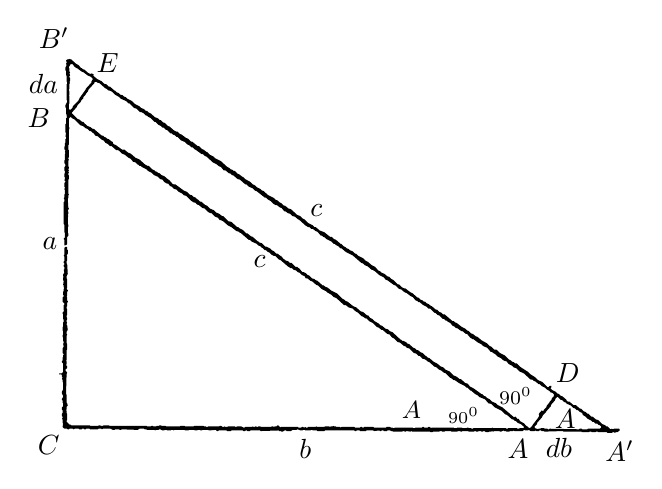
\begin{tikzpicture}[x=0.00734619cm,y=-0.00734619cm]
\fill[even odd rule] (82,85) -- (83,87) -- (83,89) -- (82,90) -- (83,93) -- (81,97) -- (81,102) -- (82,103) -- (82,110) -- (83,111) -- (83,121) -- (84,122) -- (84,125) -- (83,126) -- (83,153) -- (84,154) -- (84,156) -- (81,162) -- (81,166) -- (82,167) -- (82,177) -- (83,178) -- (83,181) -- (84,183) -- (82,185) -- (82,194) -- (81,195) -- (81,209) -- (82,210) -- (81,216) -- (82,217) -- (82,220) -- (81,221) -- (81,227) -- (80,228) -- (80,233) -- (79,234) -- (79,238) -- (81,241) -- (80,243) -- (81,245) -- (80,247) -- (80,257) -- (79,258) -- (79,262) -- (81,265) -- (81,267) -- (79,270) -- (79,275) -- (80,276) -- (80,280) -- (79,281) -- (79,286) -- (80,287) -- (80,290) -- (79,292) -- (81,294) -- (81,295) -- (79,297) -- (79,303) -- (80,304) -- (80,306) -- (79,307) -- (80,309) -- (80,316) -- (79,317) -- (79,322) -- (78,323) -- (79,325) -- (79,329) -- (78,330) -- (78,368) -- (79,369) -- (79,382) -- (80,383) -- (80,391) -- (78,393) -- (78,394) -- (79,395) -- (79,404) -- (80,405) -- (84,403) -- (84,390) -- (86,388) -- (86,384) -- (85,383) -- (85,373) -- (86,372) -- (86,369) -- (85,368) -- (85,356) -- (86,354) -- (85,353) -- (85,351) -- (86,350) -- (86,347) -- (85,345) -- (87,341) -- (86,340) -- (85,324) -- (86,323) -- (86,318) -- (87,317) -- (86,315) -- (86,291) -- (87,290) -- (87,284) -- (86,283) -- (86,280) -- (87,279) -- (86,277) -- (87,275) -- (86,273) -- (87,271) -- (87,269) -- (86,268) -- (86,258) -- (87,257) -- (86,255) -- (86,253) -- (87,252) -- (87,240) -- (86,239) -- (86,231) -- (87,230) -- (87,204) -- (88,203) -- (88,201) -- (87,200) -- (87,185) -- (89,183) -- (91,183) -- (93,185) -- (97,187) -- (107,197) -- (111,198) -- (116,202) -- (119,203) -- (123,207) -- (125,207) -- (128,210) -- (129,210) -- (133,215) -- (137,216) -- (144,222) -- (147,223) -- (150,227) -- (154,229) -- (158,233) -- (161,233) -- (169,240) -- (172,240) -- (174,241) -- (179,246) -- (184,248) -- (190,253) -- (194,255) -- (198,260) -- (202,261) -- (206,265) -- (207,265) -- (209,267) -- (211,267) -- (213,269) -- (221,273) -- (224,276) -- (230,279) -- (234,283) -- (241,286) -- (245,290) -- (249,291) -- (252,295) -- (257,298) -- (259,298) -- (262,302) -- (265,303) -- (269,307) -- (273,308) -- (277,312) -- (283,315) -- (286,318) -- (290,319) -- (299,328) -- (300,328) -- (302,330) -- (306,331) -- (309,334) -- (312,335) -- (318,340) -- (322,341) -- (328,347) -- (332,349) -- (334,349) -- (340,355) -- (345,357) -- (348,361) -- (350,361) -- (354,363) -- (362,370) -- (368,373) -- (377,380) -- (381,381) -- (383,383) -- (384,383) -- (398,395) -- (400,395) -- (403,398) -- (412,402) -- (415,405) -- (418,406) -- (421,409) -- (422,409) -- (426,413) -- (428,413) -- (431,416) -- (434,417) -- (438,421) -- (442,423) -- (444,423) -- (450,429) -- (453,430) -- (467,442) -- (468,442) -- (470,444) -- (473,444) -- (476,447) -- (480,448) -- (483,451) -- (486,452) -- (490,456) -- (495,458) -- (497,462) -- (500,462) -- (505,466) -- (508,467) -- (515,473) -- (518,474) -- (524,480) -- (532,484) -- (534,486) -- (541,490) -- (545,494) -- (550,496) -- (563,508) -- (566,508) -- (571,512) -- (578,514) -- (582,518) -- (587,521) -- (593,527) -- (596,528) -- (600,531) -- (602,531) -- (607,536) -- (613,539) -- (620,546) -- (623,547) -- (628,551) -- (630,551) -- (638,558) -- (642,559) -- (646,564) -- (650,566) -- (656,572) -- (660,573) -- (667,579) -- (669,579) -- (672,582) -- (676,583) -- (684,591) -- (688,592) -- (692,596) -- (694,596) -- (699,601) -- (701,601) -- (705,603) -- (707,605) -- (711,607) -- (720,615) -- (722,615) -- (728,620) -- (731,621) -- (736,625) -- (739,626) -- (747,634) -- (748,634) -- (753,638) -- (755,638) -- (762,643) -- (772,648) -- (775,651) -- (777,651) -- (782,656) -- (783,656) -- (790,662) -- (794,664) -- (797,667) -- (807,671) -- (813,678) -- (818,679) -- (824,685) -- (836,691) -- (842,697) -- (845,698) -- (854,706) -- (856,706) -- (858,708) -- (861,709) -- (864,712) -- (869,714) -- (875,719) -- (873,721) -- (867,721) -- (866,722) -- (863,722) -- (862,721) -- (847,721) -- (846,722) -- (844,722) -- (843,721) -- (821,721) -- (820,720) -- (818,721) -- (787,721) -- (786,722) -- (784,722) -- (783,721) -- (779,721) -- (778,720) -- (776,720) -- (775,721) -- (768,721) -- (767,720) -- (759,720) -- (758,721) -- (754,721) -- (753,720) -- (715,720) -- (714,721) -- (711,719) -- (709,719) -- (708,720) -- (702,720) -- (701,719) -- (699,719) -- (698,720) -- (687,720) -- (686,721) -- (683,721) -- (682,720) -- (651,720) -- (650,721) -- (648,721) -- (647,720) -- (644,720) -- (643,719) -- (637,719) -- (636,720) -- (615,720) -- (614,719) -- (598,719) -- (597,720) -- (595,720) -- (594,719) -- (592,719) -- (591,720) -- (582,720) -- (581,719) -- (559,719) -- (557,720) -- (556,719) -- (550,719) -- (549,718) -- (546,718) -- (545,717) -- (543,718) -- (540,718) -- (539,719) -- (537,718) -- (530,718) -- (529,719) -- (517,719) -- (515,718) -- (514,719) -- (501,719) -- (500,720) -- (497,720) -- (496,719) -- (494,720) -- (492,719) -- (490,719) -- (489,720) -- (484,720) -- (483,719) -- (454,719) -- (453,720) -- (449,716) -- (448,716) -- (446,718) -- (443,718) -- (442,719) -- (440,718) -- (438,718) -- (437,719) -- (419,719) -- (418,718) -- (415,718) -- (414,719) -- (410,718) -- (409,719) -- (407,719) -- (405,718) -- (404,719) -- (392,719) -- (391,720) -- (389,720) -- (385,718) -- (378,718) -- (377,719) -- (375,719) -- (374,718) -- (362,718) -- (361,719) -- (358,719) -- (356,718) -- (355,719) -- (353,719) -- (350,717) -- (348,717) -- (347,718) -- (328,718) -- (327,719) -- (325,719) -- (324,718) -- (321,718) -- (320,717) -- (304,717) -- (303,718) -- (288,718) -- (287,717) -- (280,717) -- (279,718) -- (255,718) -- (254,717) -- (247,717) -- (246,716) -- (244,716) -- (243,717) -- (239,717) -- (238,718) -- (233,718) -- (232,717) -- (230,717) -- (229,718) -- (222,718) -- (221,717) -- (157,717) -- (156,716) -- (147,716) -- (146,717) -- (142,717) -- (141,716) -- (139,716) -- (138,717) -- (124,717) -- (123,716) -- (91,716) -- (90,715) -- (88,715) -- (83,710) -- (83,708) -- (84,707) -- (84,696) -- (83,695) -- (83,691) -- (82,690) -- (83,688) -- (83,684) -- (85,682) -- (84,678) -- (83,677) -- (83,663) -- (82,662) -- (83,627) -- (84,625) -- (81,621) -- (81,620) -- (84,617) -- (84,614) -- (82,612) -- (83,610) -- (83,606) -- (82,604) -- (83,603) -- (83,586) -- (84,585) -- (84,575) -- (83,574) -- (83,561) -- (84,559) -- (83,558) -- (83,554) -- (85,551) -- (84,543) -- (83,542) -- (83,540) -- (84,539) -- (83,537) -- (83,534) -- (84,533) -- (84,530) -- (83,529) -- (83,526) -- (84,525) -- (84,515) -- (83,514) -- (83,511) -- (84,510) -- (84,504) -- (85,503) -- (85,501) -- (84,500) -- (84,495) -- (83,494) -- (84,492) -- (84,485) -- (85,484) -- (85,482) -- (83,480) -- (84,478) -- (84,463) -- (83,462) -- (83,458) -- (85,454) -- (84,437) -- (83,436) -- (83,432) -- (84,431) -- (84,424) -- (83,422) -- (85,419) -- (85,413) -- (84,412) -- (84,408) -- (82,407) -- (79,409) -- (79,421) -- (78,422) -- (79,424) -- (79,432) -- (78,433) -- (78,435) -- (79,436) -- (79,438) -- (78,439) -- (78,441) -- (79,442) -- (79,446) -- (78,447) -- (79,452) -- (77,455) -- (77,458) -- (78,459) -- (77,461) -- (77,465) -- (78,466) -- (77,473) -- (78,474) -- (78,477) -- (79,479) -- (78,480) -- (78,484) -- (77,485) -- (77,490) -- (78,491) -- (78,493) -- (76,495) -- (76,502) -- (79,505) -- (79,507) -- (78,508) -- (78,517) -- (79,518) -- (76,521) -- (76,523) -- (77,524) -- (77,532) -- (78,533) -- (78,537) -- (77,538) -- (77,545) -- (76,546) -- (76,552) -- (77,553) -- (77,559) -- (76,560) -- (76,563) -- (77,564) -- (77,570) -- (78,571) -- (78,574) -- (77,575) -- (78,580) -- (76,583) -- (76,591) -- (78,593) -- (78,594) -- (77,595) -- (77,598) -- (76,599) -- (76,604) -- (75,605) -- (75,607) -- (77,609) -- (77,624) -- (75,626) -- (71,626) -- (70,627) -- (70,628) -- (74,628) -- (75,629) -- (75,632) -- (76,633) -- (75,636) -- (76,637) -- (76,641) -- (77,642) -- (77,654) -- (75,658) -- (75,661) -- (77,665) -- (77,667) -- (75,670) -- (75,672) -- (76,673) -- (76,677) -- (77,678) -- (77,683) -- (75,685) -- (75,689) -- (76,690) -- (76,695) -- (75,696) -- (75,700) -- (76,701) -- (76,703) -- (75,705) -- (76,706) -- (76,712) -- (77,713) -- (76,719) -- (78,721) -- (80,722) -- (84,722) -- (85,723) -- (87,723) -- (88,722) -- (94,722) -- (95,723) -- (97,722) -- (104,722) -- (105,723) -- (109,723) -- (110,722) -- (113,722) -- (114,723) -- (116,723) -- (117,722) -- (123,722) -- (124,723) -- (137,723) -- (138,722) -- (143,722) -- (144,723) -- (146,722) -- (159,722) -- (163,724) -- (166,724) -- (167,723) -- (174,723) -- (175,724) -- (177,724) -- (178,723) -- (206,724) -- (209,722) -- (217,722) -- (218,723) -- (221,723) -- (222,724) -- (235,724) -- (236,725) -- (238,724) -- (242,724) -- (243,723) -- (245,723) -- (249,725) -- (252,725) -- (253,724) -- (256,724) -- (257,725) -- (263,725) -- (264,724) -- (267,724) -- (268,725) -- (270,724) -- (287,724) -- (288,725) -- (294,725) -- (295,724) -- (304,724) -- (305,725) -- (309,725) -- (310,724) -- (314,724) -- (315,725) -- (317,725) -- (318,724) -- (328,724) -- (329,725) -- (341,724) -- (343,726) -- (345,726) -- (346,725) -- (360,725) -- (361,726) -- (367,726) -- (368,725) -- (388,725) -- (389,726) -- (392,726) -- (393,725) -- (395,725) -- (396,726) -- (400,726) -- (401,725) -- (418,725) -- (419,726) -- (450,725) -- (451,726) -- (454,726) -- (455,727) -- (457,727) -- (460,725) -- (463,725) -- (464,726) -- (471,726) -- (474,724) -- (481,724) -- (482,723) -- (486,724) -- (487,725) -- (491,725) -- (492,724) -- (495,724) -- (496,725) -- (505,725) -- (506,724) -- (508,724) -- (509,725) -- (516,725) -- (517,726) -- (529,726) -- (530,725) -- (581,725) -- (582,726) -- (584,726) -- (585,725) -- (590,725) -- (591,726) -- (601,726) -- (602,725) -- (614,725) -- (615,726) -- (624,725) -- (625,726) -- (627,726) -- (628,725) -- (631,725) -- (632,726) -- (637,726) -- (638,725) -- (643,725) -- (644,726) -- (647,726) -- (648,727) -- (664,727) -- (665,726) -- (667,726) -- (668,727) -- (670,727) -- (671,726) -- (678,727) -- (680,726) -- (681,727) -- (712,727) -- (713,728) -- (716,728) -- (717,727) -- (728,727) -- (729,726) -- (732,726) -- (733,727) -- (737,727) -- (738,726) -- (748,726) -- (749,727) -- (759,727) -- (760,726) -- (764,726) -- (765,727) -- (767,727) -- (768,726) -- (778,726) -- (779,727) -- (788,727) -- (789,726) -- (791,726) -- (792,727) -- (795,727) -- (796,726) -- (800,726) -- (801,727) -- (803,727) -- (804,726) -- (806,726) -- (809,728) -- (813,728) -- (814,727) -- (818,727) -- (819,726) -- (821,727) -- (823,726) -- (832,726) -- (833,727) -- (835,727) -- (839,725) -- (840,726) -- (843,726) -- (844,727) -- (849,727) -- (850,726) -- (855,726) -- (856,725) -- (858,726) -- (872,726) -- (875,724) -- (877,725) -- (881,725) -- (883,724) -- (886,726) -- (893,726) -- (894,725) -- (896,726) -- (900,726) -- (901,725) -- (904,725) -- (905,726) -- (909,726) -- (910,727) -- (942,726) -- (943,727) -- (974,727) -- (975,728) -- (987,728) -- (988,727) -- (991,727) -- (992,728) -- (998,728) -- (999,727) -- (1002,727) -- (1003,728) -- (1018,728) -- (1019,729) -- (1027,729) -- (1028,728) -- (1030,728) -- (1032,729) -- (1033,728) -- (1036,728) -- (1040,725) -- (1040,723) -- (1039,722) -- (1030,722) -- (1029,723) -- (1026,722) -- (1024,723) -- (1019,718) -- (1017,718) -- (1015,716) -- (1010,714) -- (1003,707) -- (999,706) -- (993,701) -- (991,701) -- (986,696) -- (984,696) -- (981,693) -- (978,692) -- (973,687) -- (971,687) -- (964,681) -- (960,681) -- (953,675) -- (950,675) -- (948,673) -- (948,672) -- (941,666) -- (938,665) -- (935,662) -- (932,661) -- (929,658) -- (923,655) -- (920,652) -- (922,650) -- (922,648) -- (919,648) -- (917,650) -- (915,650) -- (906,641) -- (899,638) -- (894,633) -- (886,628) -- (882,624) -- (868,615) -- (862,609) -- (859,609) -- (857,607) -- (854,606) -- (852,604) -- (848,602) -- (841,595) -- (833,591) -- (828,586) -- (826,585) -- (823,585) -- (818,580) -- (815,579) -- (810,574) -- (801,569) -- (794,563) -- (791,562) -- (786,558) -- (783,557) -- (779,553) -- (776,552) -- (773,549) -- (767,546) -- (758,539) -- (755,538) -- (753,536) -- (751,536) -- (737,524) -- (734,524) -- (731,521) -- (728,520) -- (724,516) -- (722,516) -- (715,510) -- (714,510) -- (709,506) -- (706,505) -- (703,502) -- (701,502) -- (699,500) -- (696,499) -- (692,495) -- (690,495) -- (682,488) -- (678,486) -- (669,479) -- (667,479) -- (663,477) -- (658,472) -- (656,472) -- (649,465) -- (645,463) -- (641,459) -- (639,459) -- (633,454) -- (628,452) -- (626,450) -- (622,448) -- (617,442) -- (611,439) -- (604,433) -- (600,431) -- (596,427) -- (588,423) -- (584,419) -- (582,419) -- (578,415) -- (573,413) -- (571,411) -- (568,410) -- (566,408) -- (562,406) -- (558,402) -- (557,402) -- (549,395) -- (546,394) -- (542,390) -- (539,390) -- (529,382) -- (521,379) -- (514,373) -- (512,373) -- (509,370) -- (501,366) -- (495,360) -- (491,358) -- (487,354) -- (482,352) -- (471,342) -- (467,341) -- (461,336) -- (459,336) -- (455,332) -- (451,330) -- (448,327) -- (445,326) -- (442,323) -- (432,318) -- (423,310) -- (421,310) -- (418,307) -- (412,304) -- (409,301) -- (405,299) -- (401,295) -- (392,290) -- (388,286) -- (387,286) -- (382,282) -- (379,281) -- (374,276) -- (372,276) -- (370,274) -- (367,273) -- (365,271) -- (361,269) -- (350,259) -- (340,254) -- (337,251) -- (331,248) -- (326,243) -- (325,243) -- (320,239) -- (317,238) -- (312,233) -- (310,233) -- (300,225) -- (298,225) -- (293,220) -- (290,219) -- (282,213) -- (279,212) -- (275,208) -- (273,208) -- (269,206) -- (261,199) -- (258,198) -- (253,193) -- (250,192) -- (246,188) -- (244,188) -- (241,185) -- (236,183) -- (228,176) -- (225,175) -- (222,172) -- (220,172) -- (217,169) -- (212,167) -- (209,164) -- (201,160) -- (196,155) -- (188,151) -- (185,148) -- (182,147) -- (180,145) -- (176,144) -- (173,141) -- (170,140) -- (167,137) -- (166,137) -- (158,130) -- (156,130) -- (152,126) -- (148,125) -- (144,121) -- (136,117) -- (129,111) -- (130,109) -- (129,109) -- (127,107) -- (124,108) -- (120,106) -- (113,100) -- (111,100) -- (109,98) -- (108,98) -- (104,93) -- (100,91) -- (91,83) -- (87,82) -- (86,83) -- (84,83) -- cycle
(893,718) -- (897,714) -- (897,712) -- (905,703) -- (907,699) -- (913,693) -- (913,692) -- (921,683) -- (921,681) -- (928,673) -- (929,670) -- (932,667) -- (933,667) -- (938,672) -- (940,672) -- (944,676) -- (946,676) -- (949,679) -- (956,682) -- (960,686) -- (963,687) -- (966,690) -- (968,690) -- (971,693) -- (974,694) -- (976,696) -- (976,698) -- (981,701) -- (985,705) -- (991,708) -- (993,710) -- (995,710) -- (998,713) -- (1001,713) -- (1003,715) -- (1006,716) -- (1008,718) -- (1008,720) -- (1006,722) -- (985,722) -- (984,723) -- (975,723) -- (974,722) -- (971,722) -- (970,723) -- (919,722) -- (918,723) -- (916,723) -- (915,722) -- (910,722) -- (909,721) -- (904,721) -- (903,722) -- (900,722) -- (898,723) -- (897,722) -- (895,722) -- (893,720) -- cycle
(92,175) -- (100,166) -- (102,162) -- (107,157) -- (109,153) -- (112,150) -- (112,148) -- (116,144) -- (116,143) -- (120,138) -- (121,135) -- (131,124) -- (131,123) -- (132,122) -- (135,122) -- (136,123) -- (140,124) -- (150,133) -- (151,133) -- (156,137) -- (158,137) -- (162,139) -- (167,144) -- (174,148) -- (177,151) -- (186,155) -- (190,159) -- (192,159) -- (200,167) -- (204,168) -- (210,174) -- (212,174) -- (216,176) -- (220,180) -- (222,180) -- (224,182) -- (228,184) -- (235,191) -- (237,191) -- (242,196) -- (246,198) -- (249,201) -- (251,201) -- (255,205) -- (257,205) -- (263,211) -- (265,211) -- (267,213) -- (270,214) -- (273,217) -- (275,217) -- (281,223) -- (288,226) -- (292,230) -- (296,232) -- (299,235) -- (301,235) -- (305,239) -- (306,239) -- (317,247) -- (319,247) -- (322,250) -- (325,251) -- (336,261) -- (342,264) -- (347,268) -- (350,269) -- (355,275) -- (358,275) -- (364,280) -- (366,280) -- (369,283) -- (372,284) -- (379,290) -- (383,291) -- (392,299) -- (394,299) -- (398,303) -- (405,306) -- (409,310) -- (412,311) -- (426,322) -- (428,322) -- (431,325) -- (436,328) -- (441,333) -- (445,335) -- (447,335) -- (452,339) -- (455,340) -- (460,346) -- (462,346) -- (466,349) -- (470,350) -- (474,354) -- (478,355) -- (484,360) -- (485,360) -- (496,370) -- (501,373) -- (503,373) -- (506,376) -- (509,376) -- (514,380) -- (517,381) -- (523,388) -- (525,388) -- (527,390) -- (530,391) -- (533,394) -- (541,398) -- (545,402) -- (547,402) -- (549,404) -- (553,406) -- (557,410) -- (559,410) -- (566,416) -- (578,422) -- (593,435) -- (596,436) -- (599,439) -- (604,441) -- (611,447) -- (613,447) -- (615,449) -- (616,449) -- (624,456) -- (632,460) -- (635,464) -- (638,465) -- (649,473) -- (652,474) -- (658,480) -- (662,481) -- (668,486) -- (671,487) -- (679,493) -- (682,494) -- (687,500) -- (690,501) -- (692,503) -- (694,503) -- (700,508) -- (706,511) -- (709,514) -- (712,514) -- (719,521) -- (722,522) -- (725,525) -- (728,526) -- (734,532) -- (736,532) -- (739,535) -- (741,535) -- (743,537) -- (747,539) -- (751,544) -- (754,545) -- (757,548) -- (759,548) -- (766,553) -- (768,553) -- (774,558) -- (776,558) -- (782,565) -- (783,565) -- (785,567) -- (787,567) -- (795,573) -- (801,576) -- (804,579) -- (811,582) -- (817,589) -- (819,589) -- (821,591) -- (825,593) -- (829,597) -- (835,600) -- (838,603) -- (842,605) -- (844,605) -- (848,610) -- (854,613) -- (857,616) -- (861,617) -- (867,623) -- (874,626) -- (886,637) -- (889,637) -- (891,639) -- (894,640) -- (900,645) -- (902,645) -- (905,648) -- (911,651) -- (914,654) -- (919,657) -- (920,659) -- (924,660) -- (926,662) -- (926,666) -- (923,669) -- (922,672) -- (919,675) -- (919,676) -- (914,682) -- (913,685) -- (909,689) -- (909,690) -- (908,691) -- (906,691) -- (905,690) -- (905,691) -- (901,695) -- (900,697) -- (901,699) -- (899,703) -- (889,716) -- (889,717) -- (885,721) -- (882,720) -- (879,717) -- (878,717) -- (875,713) -- (868,709) -- (866,707) -- (866,705) -- (863,705) -- (860,701) -- (857,702) -- (837,685) -- (829,681) -- (826,678) -- (819,675) -- (815,671) -- (811,669) -- (808,666) -- (805,665) -- (802,662) -- (801,662) -- (787,652) -- (781,649) -- (777,644) -- (773,643) -- (765,636) -- (763,636) -- (758,632) -- (753,630) -- (746,623) -- (739,620) -- (735,616) -- (730,614) -- (724,609) -- (718,606) -- (711,600) -- (708,599) -- (705,596) -- (704,596) -- (699,591) -- (696,590) -- (691,586) -- (689,586) -- (686,583) -- (683,582) -- (675,575) -- (673,575) -- (670,572) -- (666,570) -- (664,570) -- (662,568) -- (661,568) -- (647,555) -- (642,553) -- (639,550) -- (635,549) -- (629,544) -- (626,543) -- (623,540) -- (616,536) -- (612,532) -- (608,530) -- (605,526) -- (603,526) -- (596,520) -- (592,519) -- (584,512) -- (579,510) -- (569,502) -- (566,501) -- (564,499) -- (560,497) -- (551,488) -- (541,483) -- (535,478) -- (530,476) -- (528,474) -- (526,474) -- (517,466) -- (514,465) -- (512,463) -- (508,462) -- (503,457) -- (500,456) -- (497,453) -- (493,451) -- (491,451) -- (485,444) -- (484,444) -- (482,442) -- (479,442) -- (472,435) -- (469,435) -- (466,432) -- (462,431) -- (460,429) -- (459,429) -- (454,423) -- (453,423) -- (448,419) -- (446,419) -- (442,415) -- (438,413) -- (435,410) -- (429,407) -- (427,407) -- (421,401) -- (417,400) -- (415,398) -- (414,398) -- (405,390) -- (402,389) -- (396,384) -- (394,384) -- (388,378) -- (382,375) -- (380,373) -- (378,373) -- (368,364) -- (363,363) -- (354,354) -- (352,354) -- (347,350) -- (342,348) -- (338,344) -- (331,341) -- (326,336) -- (323,335) -- (316,329) -- (314,329) -- (310,325) -- (309,325) -- (306,322) -- (303,321) -- (300,318) -- (296,317) -- (291,312) -- (286,310) -- (271,299) -- (268,299) -- (266,298) -- (260,291) -- (259,291) -- (252,285) -- (247,283) -- (244,280) -- (241,279) -- (239,277) -- (237,277) -- (235,275) -- (231,273) -- (225,267) -- (223,267) -- (219,265) -- (209,256) -- (202,253) -- (194,246) -- (189,244) -- (183,239) -- (179,239) -- (168,231) -- (165,230) -- (163,228) -- (163,226) -- (162,225) -- (161,225) -- (156,221) -- (153,220) -- (151,218) -- (148,217) -- (146,215) -- (144,215) -- (130,203) -- (128,203) -- (124,200) -- (119,198) -- (116,195) -- (115,195) -- (112,191) -- (110,191) -- (105,187) -- (102,186) -- (92,176) -- cycle
(93,91) -- (95,93) -- (95,94) -- (100,98) -- (101,98) -- (109,104) -- (112,105) -- (120,111) -- (125,113) -- (128,116) -- (128,118) -- (126,121) -- (126,123) -- (116,134) -- (116,135) -- (106,149) -- (103,155) -- (94,164) -- (93,167) -- (90,170) -- (88,170) -- (87,169) -- (87,160) -- (88,159) -- (88,147) -- (87,146) -- (88,144) -- (88,138) -- (87,137) -- (87,135) -- (88,134) -- (88,125) -- (89,124) -- (88,122) -- (89,120) -- (89,115) -- (88,114) -- (88,112) -- (89,111) -- (88,107) -- (89,105) -- (88,104) -- (88,99) -- (87,98) -- (87,96) -- (90,91) -- cycle;
\node[inner sep=0pt,font=\fontsize{10}{12}\selectfont] at (61,46) {$B'$};
\node[inner sep=0pt,font=\fontsize{10}{12}\selectfont] at (154,90) {$E$};
\node[inner sep=0pt,font=\fontsize{10}{12}\selectfont] at (43,126) {$da$};
\node[inner sep=0pt,font=\fontsize{10}{12}\selectfont] at (35,185) {$B$};
\node[inner sep=0pt,font=\fontsize{10}{12}\selectfont] at (54,401) {$a$};
\node[inner sep=0pt,font=\fontsize{10}{12}\selectfont] at (515,345) {$c$};
\node[inner sep=0pt,font=\fontsize{10}{12}\selectfont] at (417,433) {$c$};
\node[inner sep=0pt,font=\fontsize{10}{12}\selectfont] at (950,626) {$D$};
\node[inner sep=0pt,font=\fontsize{7}{9}\selectfont] at (860,665) {$90^{0}$};
\node[inner sep=0pt,font=\fontsize{6}{8}\selectfont] at (770,700) {$90^{0}$};
\node[inner sep=0pt,font=\fontsize{9}{11}\selectfont] at (680,690) {$A$};
\node[inner sep=0pt,font=\fontsize{10}{12}\selectfont] at (946,706) {$A$};
\node[inner sep=0pt,font=\fontsize{10}{12}\selectfont] at (52,751) {$C$};
\node[inner sep=0pt,font=\fontsize{10}{12}\selectfont] at (496,757) {$b$};
\node[inner sep=0pt,font=\fontsize{10}{12}\selectfont] at (864,757) {$A$};
\node[inner sep=0pt,font=\fontsize{10}{12}\selectfont] at (935,756) {$db$};
\node[inner sep=0pt,font=\fontsize{10}{12}\selectfont] at (1040,760) {$A'$};
\end{tikzpicture}


Fig. 8.
\end{minipage}\end{center}
